\documentclass[letter,10pt,twocolumn,openany]{dndbook}

% Use babel or polyglossia to automatically redefine macros for terms
% Armor Class, Level, etc...
% Default output is in English; captions are located in lib/dndstring-captions.sty.
% If no captions exist for a language, English will be used.
%1. To load a language with babel:
%	\usepackage[<lang>]{babel}
%2. To load a language with polyglossia:
%	\usepackage{polyglossia}
%	\setdefaultlanguage{<lang>}
\usepackage[english]{babel}
% For further options (multilanguage documents, hypenations, language environments...)
% please refer to babel/polyglossia's documentation.

\usepackage[utf8]{inputenc}
\usepackage[singlelinecheck=false]{caption}
\usepackage{lipsum}
\usepackage{listings}
\usepackage{shortvrb}
\usepackage{stfloats}
\usepackage{hyperref}

\captionsetup[table]{labelformat=empty,font={sf,sc,bf,},skip=0pt}

\MakeShortVerb{|}

\lstset{%
  basicstyle=\ttfamily,
  language=[LaTeX]{TeX},
  breaklines=true,
}

\title{Homebrew\\
for D\&D 5e}
\author{Jens Keim}
\date{2019/11/27}

\begin{document}

\frontmatter

\maketitle

\tableofcontents

\mainmatter

\chapter{Character Specialized}

\section{Magic Items}

\DndItemHeader{Dagger of Disinterest}{Weapon (dagger), unknown rarity (requires attunement)}
You gain a +2 bonus to attack and damage rolls made with this magic weapon.\\

This magic weapon has 3 charges. When you hit an enemy with this weapon, you can choose to expend one of its charges to heal you or an allied creature within 60 feet by half the damage done by your attack rounded down plus the creatures constitution modifier.\\
The dagger regains 1d3 expended charges daily at dawn. If you healed yourself with its abilities on the day before, half the result of the recharge dice and round down.\\

%DM only
%\subparagraph{Curse} This dagger is cursed. If you heal yourself, your maximum hit points reduce by the amount of hit points you healed yourself with the dagger this day after your next long rest (after you regained your hit points from your rest). If you are reduced to 0 hit points by this, you crumble to ash and are contained in the dagger. You can be freed and resurrectted with the remove curse spell.\\
%This curse can not be detected by the identify spell until the caster saw someone die this way and is looking for the cause of it.

\begin{figure}
    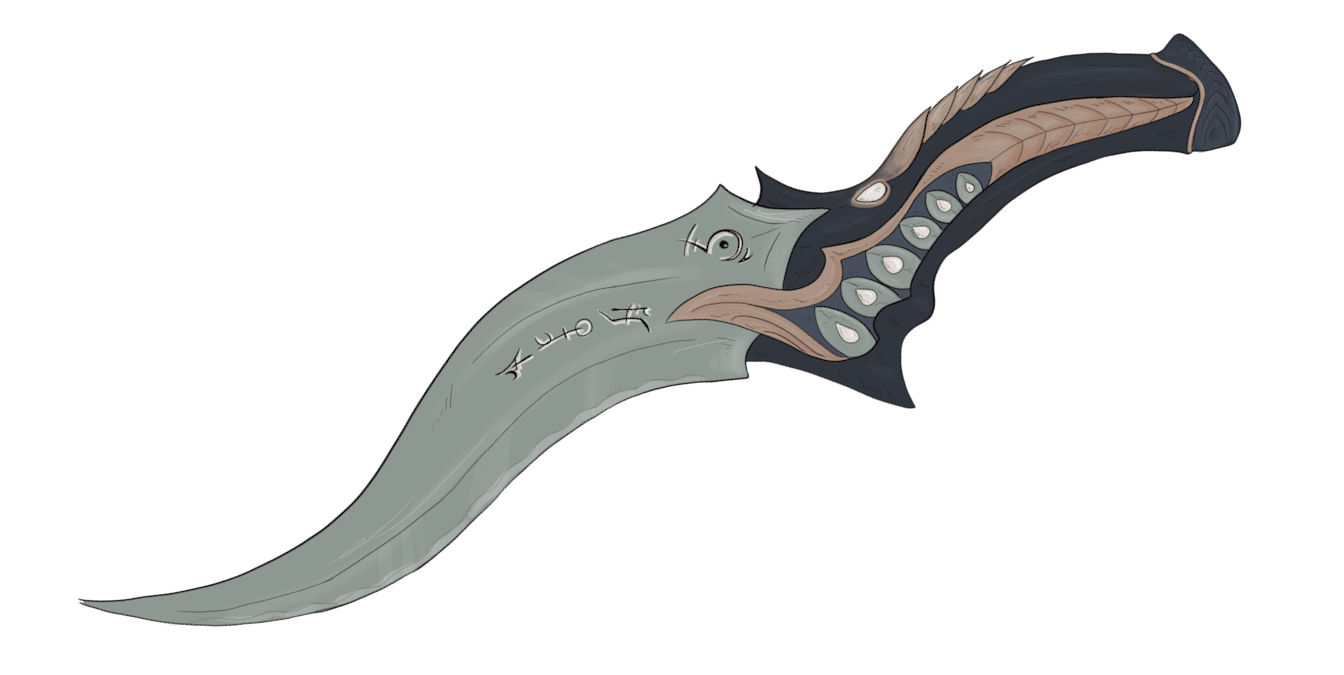
\includegraphics[width=9cm]{images/dagger_of_disinterest.png}
    \caption{Dagger of Disinterest}
\end{figure}

\DndItemHeader{Druid Totem}{Wonderous item, unknown rarity (requires attunement by a druid)}

This magic item is a small locket made of wood, that appears like a small animal of the owners choice. Though most druids change it to the animal they wild shape to.\\
One can embed multiple gems to it. Embedding a gem, counts as attuning to the gem. Once a gem is embedded into the totem it can not be removed again.\\

\subparagraph{Water Gem} This magic sarphire has 3 charges. During your wild shape, you might expend one of its charges to activate the following effect.\\
Each creature you hit during your next attack action passes 2d6 hit points to the next creature that hits it. Meaning the creature you attacked looses those hitpoints and the creature hitting it gains those hit points.\\

The totem regains 1d3 expended charges daily at dawn. Those charges are mutually assigned to a random Gem, that can regain charges.

\begin{figure}
    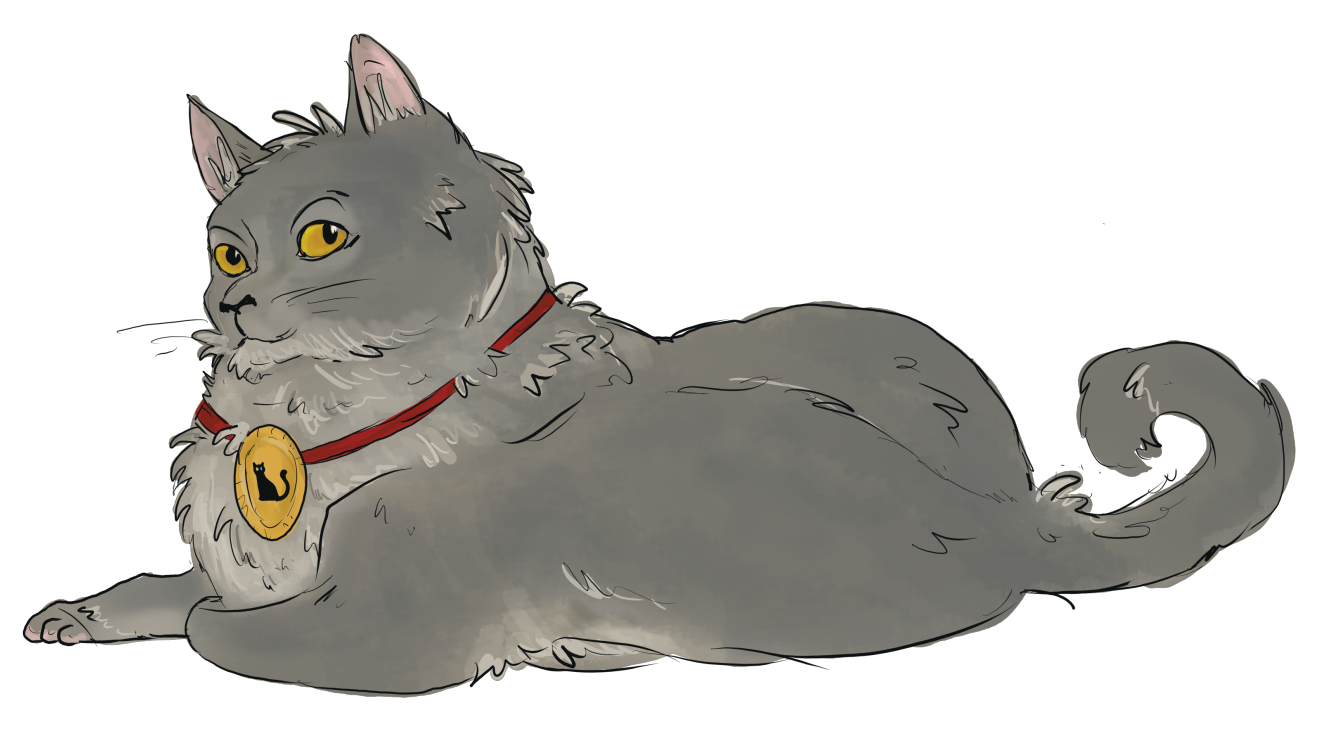
\includegraphics[width=9cm]{images/cat.png}
    \caption{A cat wearing the druid totem. She is not a druid, she just likes the locket.}
\end{figure}

\begin{figure}
    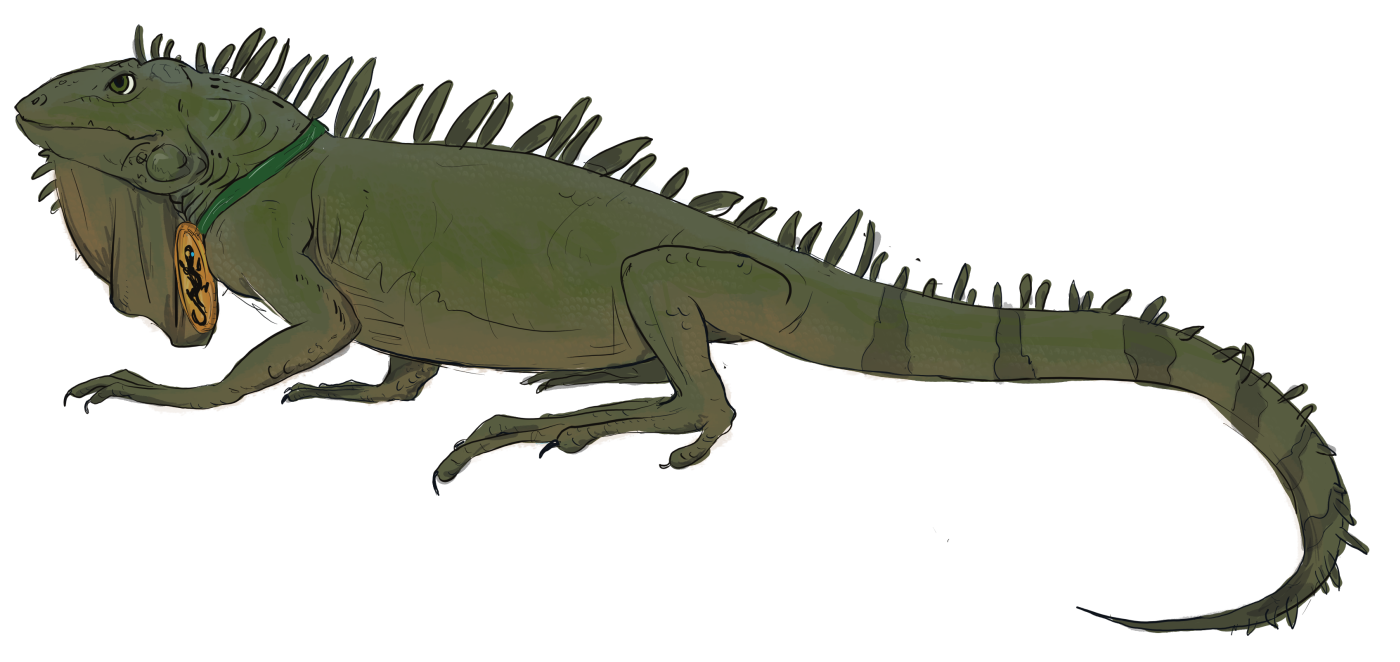
\includegraphics[width=9cm]{images/iguana.png}
    \caption{A druid in his natural habitat sunning himself, while wearing the druid totem.}
\end{figure}

\begin{figure}
    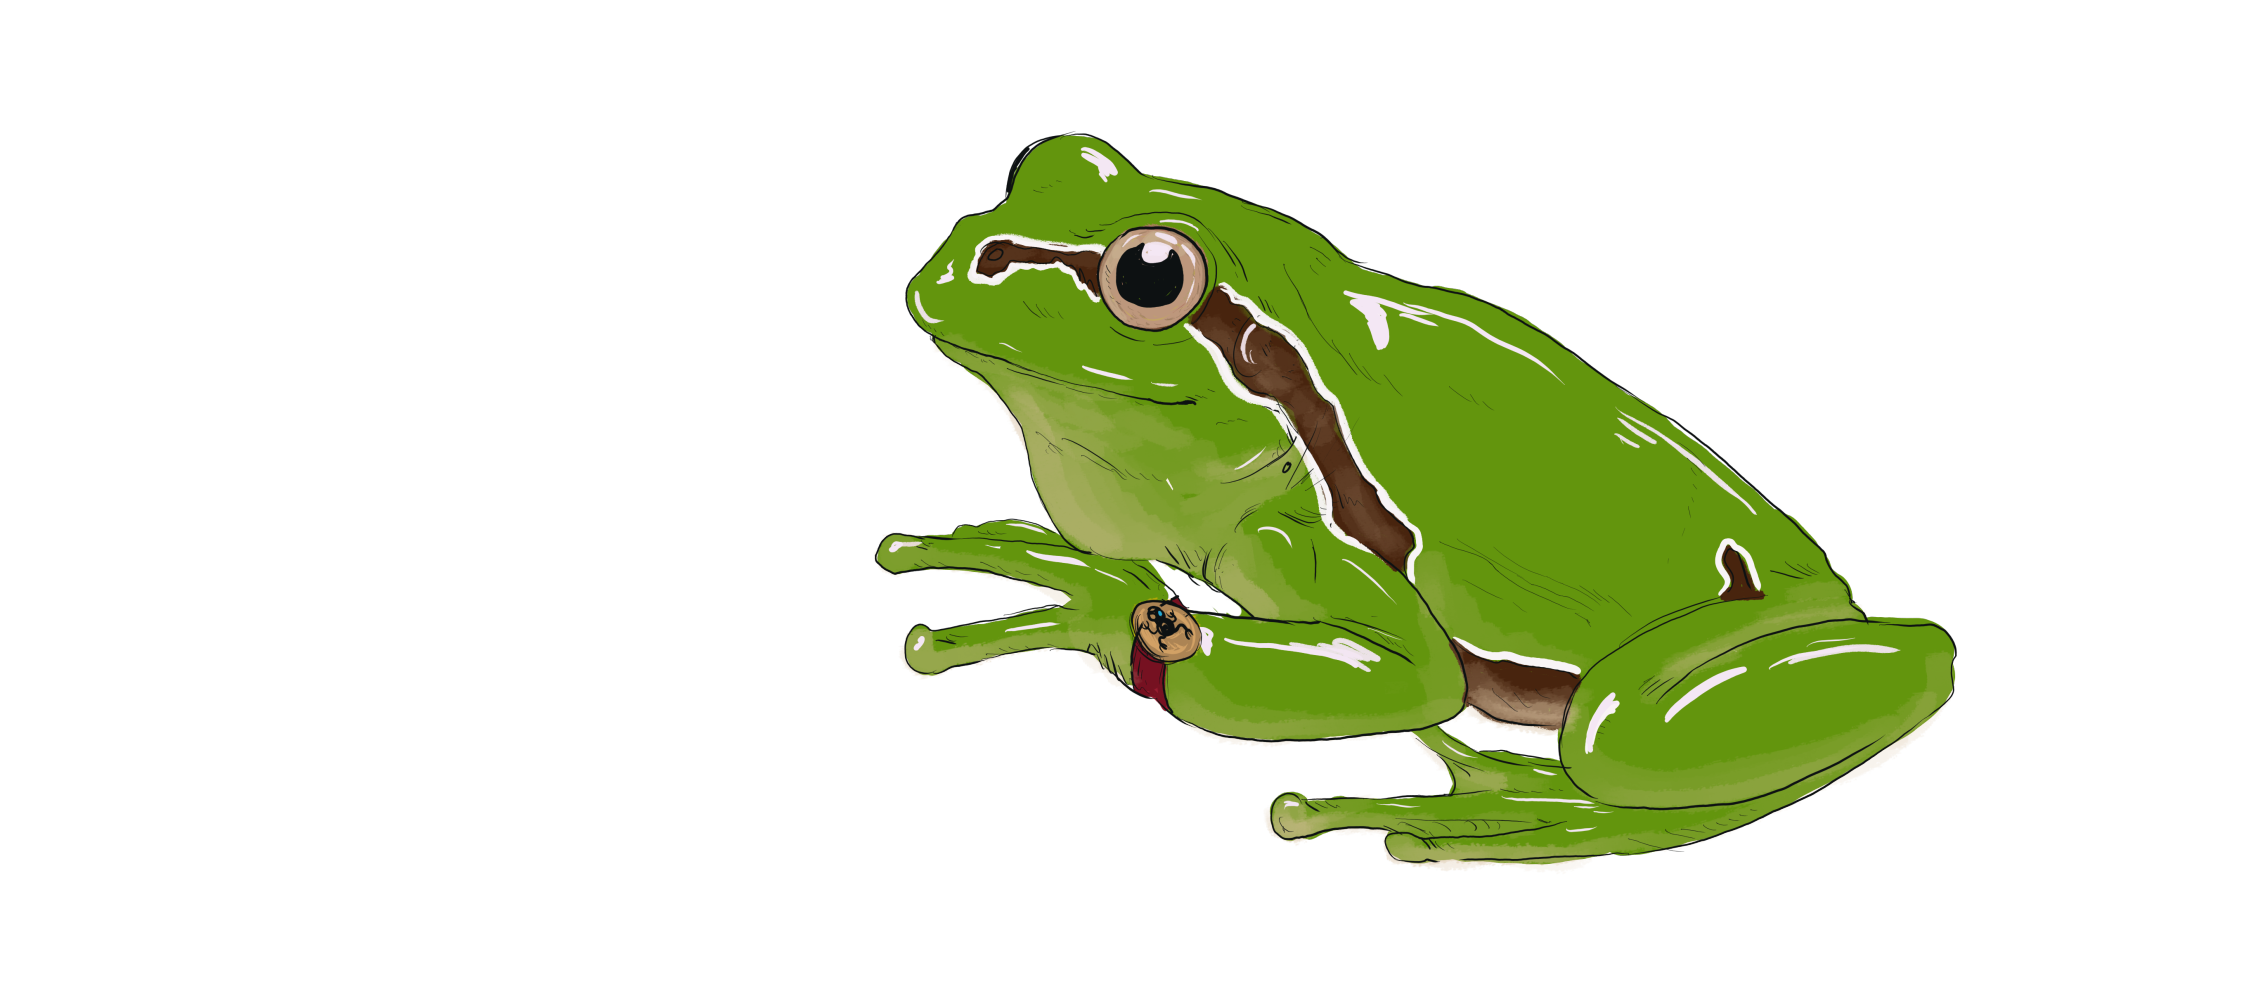
\includegraphics[width=9cm]{images/frog.png}
    \caption{A druid wild shaped into a frog wearing the druid totem.}
\end{figure}

\begin{figure}
    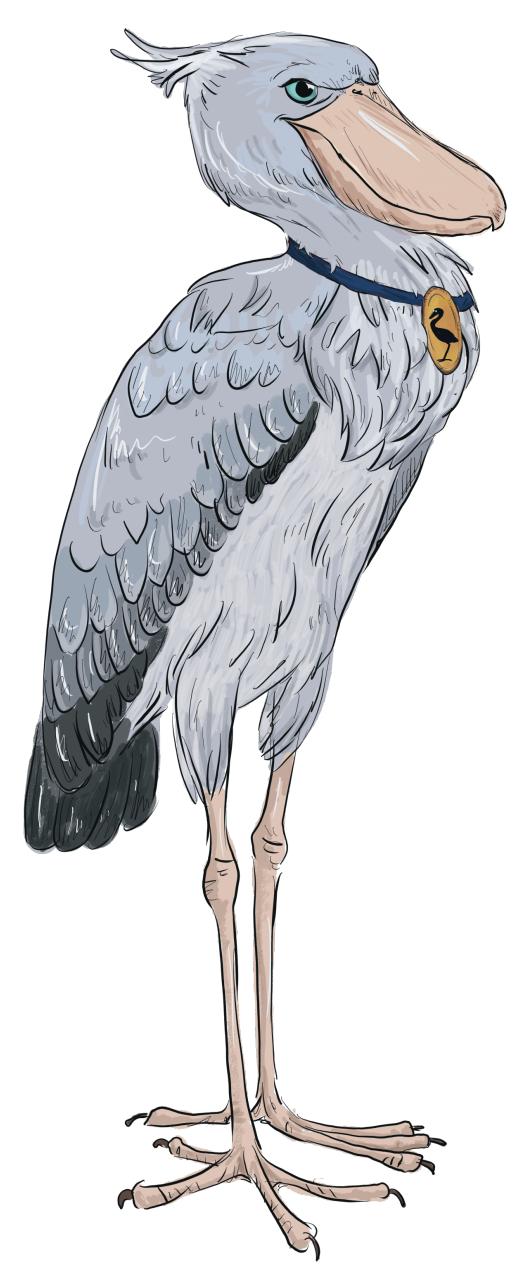
\includegraphics[width=9cm]{images/shoebill.png}
    \caption{A druid wearing the druid totem, while wild shaped into a shoebill.}
\end{figure}

\DndItemHeader{Fey Scroll}{Scroll, unknown rarity (requires attunement by a warlock)}

A fey scroll works just like a spell scroll. In addition if you can attune to it, you can merge it with your book of shadows. The scroll is then mended into the book. This consumes the scroll, meaning it is no longer an item on its own.\\
Non-ritual spells are known to the books owner, once they were added to the book in this way and only this way.\\
If the scroll merged into your book of shadows in this way, contains an eldritch invocation the owner of the book gains that invocation in addition to the invocations he already knows. Invocations gained this way can not be replaced, when the owner of the book gains a level.

\DndItemHeader{Manual of Maneuvers, Volume 3}{Wondrous item, unknown rarity (requires a battle master)}
This book describes Maneuver exercises, and its words are charged with magic. If you spend 24 hours over a period of 6 days or fewer studying the book's contents and practicing its guidelines, you gain the Maneuver discribed below. The manual then loses its magic, but regains it in ten years.\\

\subparagraph{Fearless Rescue}

»One of your allies falls, and without regard for your own wellbeing, you rush to make the attacker pay. Your bravery inspires your ally to fight on.«\\

Once per short rest when an enemy within 30 feet of you reduces an ally below 10 hit points, you can as a Reaction expend a superiority die to move to the nearest square from which you can attack that enemy and attack that enemy. You add the superiority die to the attack's damage roll.

The ally then regains 1d6 hit points and 1d6 hit points more for every opportunity attack you provoke while moving to the target.

\begin{figure}
    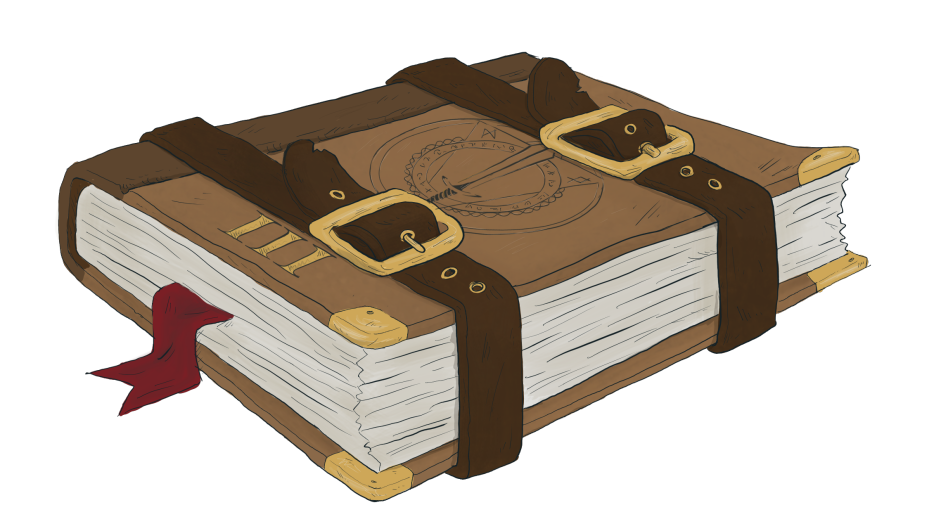
\includegraphics[width=9cm]{images/manual_of_maneuvers.png}
    \caption{Manual of Meneuvers}
\end{figure}

\DndItemHeader{Zinlee's Amulet of Commoner Protection}{Wondrous item, uncommon}
Wearing this item raises the maximum HP of the wearer to 25
If the wearer has more then 25 maximum HP it has no effect.

\section{Spells}

Fey Hex works like the normal hex spell, but gives disadvantage on attack rolls or saving throws (your choice) [instead of ability checks] until the end of your next turn.

\DndSpellHeader%
  {Fey Hex}
  {3rd-level enchantment}
  {1 bonus action}
  {90 feet}
  {V, S, M (the petrified eye of a pixie)}
  {Concentration, up to 1 minute}

You place a curse on a creature that you can see within range. Until the spell ends you deal an extra 1d6 necrotic damage to the target whenever you hit it with an attack. The target has disadvantage on attack rolls or saving throws (your choice) until the end of your next turn.\\
If the target drops to 0 hit points before this spell ends. you can use a bonus action on a subsequent turn of yours to curse a new creature.\\
A remove curse cast on the target ends this spell early.\\
At Higher Levels. When you cast this spell using a spell slot of 5th level, you can maintain your concentration on the spell for up to 1 hour.

\section{Eldritch Invocation}

\DndItemHeader{Bouncing Blast}{Prerequisite: eldritch blast cantrip}

When you hit a creature with eldritch blast, once per short rest you can spread the damage onto the creatures around it.\\
The creature you hit gets full damage, while each creature within 5 feet of it gets half that damage, as long as their AC is lower or equal to your attack roll.

\begin{figure}
    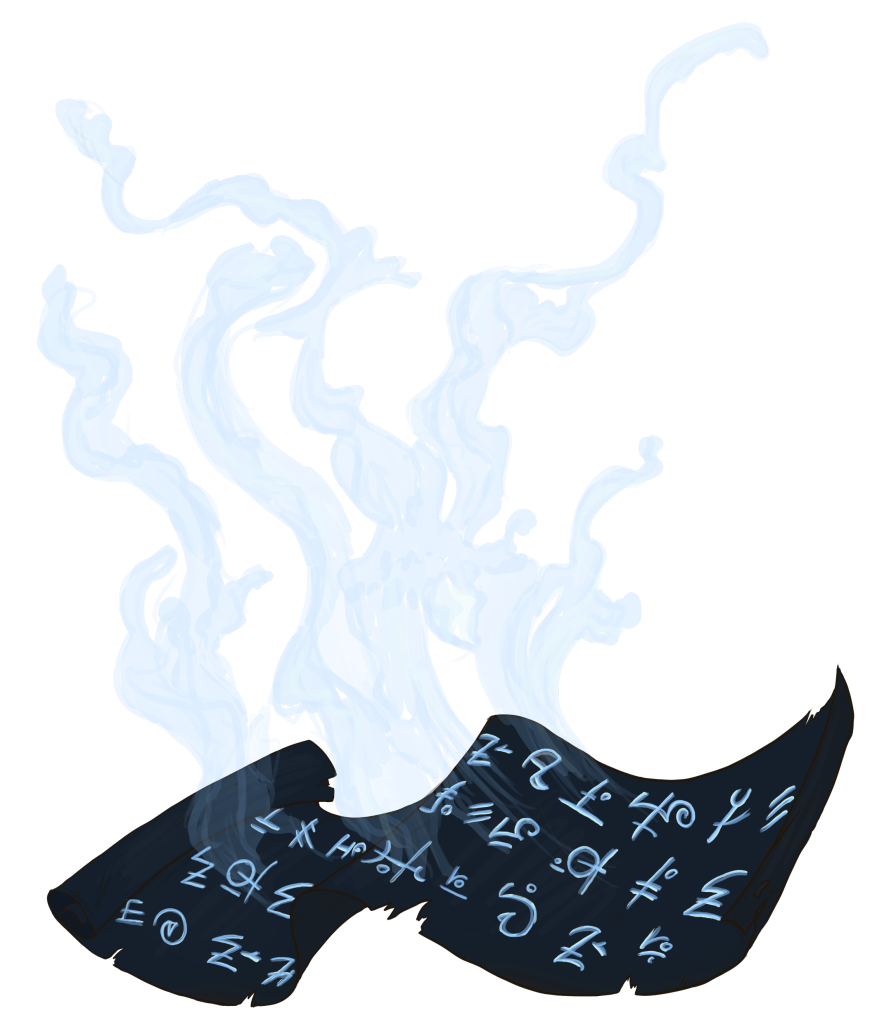
\includegraphics[width=9cm]{images/fey_scroll.png}
    \caption{Fey Scroll}
\end{figure}

\chapter{Special Features}

\subsection{Power of a Water Guardian}

Once per day, you can use a short rest to meditate as the guardian showed you. You make a Wisdom Check. If the result is 10 or higher you can use the \textbf{Frost Jab} Action once until the end of your next long rest. If the result is 15 or higher you instead can use the \textbf{Frost Kick} Action instead.

\paragraph{Frost Jab} Melee Weapon Attack str/dex to hit, reach 5ft., one target. Hit: 1d8+str/dex bludgeoning damage plus 3d6 cold damage.

\paragraph{Frost Kick} Melee Weapon Attack str/dex to hit, reach 5ft., one target. Hit: 2d6+str/dex bludgeoning damage plus 4d6 cold damage. If the target is a creature, it must succeed a Strength saving throw or be knocked prone, the DC of which is the result of your attack roll or 15, whatever is the lowest.

\backmatter

\section{Credits}

\paragraph{Drawings} Anne Wilderotter
\paragraph{Magic Items} Jens Keim
\paragraph{Spells} Jens Keim
\paragraph{Invocations} Jens Keim

\section{Licensing}

This document is licensed under \href{https://creativecommons.org/licenses/by-sa/4.0/legalcode}{\textbf{Creative Commons Attribution Share Alike 4.0 International}}.

\end{document}
